% For help on subfiles see https://www.sharelatex.com/learn/Multi-file_LaTeX_projects
\documentclass[../main.tex]{subfile}


\begin{document}
	\paragraph{} Smartphones had become an integral part of our lives. We use it for communication, financial transcations, entertainment and many other activities. Past several years have seen an increase in the number of malwares targeted toward smartphones and it is still increasing. The major target of such malwares are the smartphones running Android. Due to the high number of Android apps created or modified everyday, its impossible to analyze them manually for malicious behavior and thus the need for good automatic malware analysis tools and techniques is arises. Google is already using some automatic tools to analyze every app uploaded to Google Play Store but hackers always comes up with new ways to fool the system and thus enable themselves to upload malwares to Google Playstore. Therefore it is very important to have the tools to analyze android samples for malicious behavior even though they are analyzed before. In this project we worked on developing the tools that will allow analysts to analyze samples dynamically or statically.
	\paragraph{} In this chapter we will discuss some fundamental concepts related to android applications and android malware analysis.
	
	\section{Android application fundamentals}\label{sec:app_fundamentals}
		\paragraph{} Android application are mostly written in Java. The Android SDK tool compile this code along with any data and resources files into an APK, an Android Package. One APK file contain all contents of an Android app and is the file that Android devices use to install the application \cite{app_fundamentals}. We will discuss the structure of an APK file in section \ref{sec:apk}. In this section we will discuss some basic parts of an Android application.
		
		\subsection{Application components}
		\paragraph{} The essential building blocks of an Android application are called App components. Each component is an entry point to the application. Each type serves a distinct purpose and has a distinct life-cycle that defines how the component is created and destroyed. The communication between these components (except Content providers) is done using messages called "Intents" (section \ref{sec:intents}). It is also important to note that all of these components needs to be listed in AndroidManifest.xml file, for more detailed description of this file please look at section \ref{sec:apk_file_contents}. There are four different types of app components:
			\begin{itemize}
				\item \textbf{Activities} An activity is the entry point for interacting with the user. It represents a single screen with a user interface. Each activity is independent from others \cite{app_fundamentals}.
				\item \textbf{Services} A service is a general-purpose entry point for keeping an app running in the background for all kinds of reasons. It is a component that runs in the background to perform long-running operations or to perform work for remote processes. A service does not provide a user interface\cite{app_fundamentals}. 
				\item \textbf{Broadcast receivers} A broadcast receiver is a component that enables the system to deliver events to the app outside of a regular user flow, allowing the app to respond to system-wide broadcast announcements. Because broadcast receivers are another well-defined entry into the app, the system can deliver broadcasts even to apps that aren't currently running. Although broadcast receivers don't display a user interface, they may create a status bar notification to alert the user when a broadcast event occurs. More commonly, though, a broadcast receiver is just a gateway to other components and is intended to do a very minimal amount of work \cite{app_fundamentals}.
				\item \textbf{Content providers} A content provider manages a shared set of app data that you can store in the file system, in a SQLite database, on the web, or on any other persistent storage location that your app can access. Through the content provider, other apps can query or modify the data if the content provider allows it. For example, the Android system provides a content provider that manages the user's contact information. As such, any app with the proper permissions can query the content provider, such as ContactsContract.Data, to read and write information about a particular person \cite{app_fundamentals}.
			\end{itemize}
		\subsection{Intents messages}\label{sec:intents}
			\paragraph{} Three of the four component types activities, services, and broadcast receivers can be activated by an asynchronous message called an intent. Intents bind individual components to each other at runtime. You can think of them as the messengers that request an action from other components, whether the component belongs to your app or another \cite{app_fundamentals}. Although intents facilitate communication between components in several ways, there are three fundamental use cases:
				\begin{itemize}
					\item Starting an activity
					\item Starting a service
					\item Delivering a broadcast
				\end{itemize}
			\paragraph{} Readers more interested in this topic are recommend to have a look at \cite{intents}.
			
			
	\section{APK file}\label{sec:apk}	
		\paragraph{} Android Application Package(APK) is the file format used for an android application. It contains all the resources required for an application to run on android operating system. Its basically a zip file or a jar file with extension of ".apk"\cite{APK_structure}.
		
		\subsection{APK file contents} \label{sec:apk_file_contents}
		\paragraph{} Normally an apk file contains following files or folders:
		
		\begin{figure}[h]
			\centering
			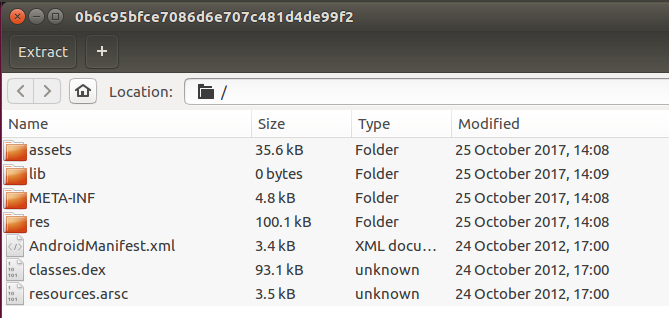
\includegraphics[width=\textwidth]{apk_contents.png}
			\caption{Files inside an APK}
		\end{figure}
		
		\begin{itemize}
			\item \textbf{assets/:} It provides a way to include arbitrary files like text, xml, fonts, music and video in your application and allow you to access your data raw/untouched. AssetManager is used to read this data\cite{android_assets}. Due to raw access sometimes this directory contains executable payloads and dynamically loaded code. One interesting usage is storing Dex files in it to avoid its reverse engineering. \cite{lim2016android}
			
			\item \textbf{lib/:} This directory is for natively compiled code. This directory contains a subdirectory for each platform type, like armeabi, armeabi-v7a, arm64-v8a, x86, x86\textunderscore64, and mips \cite{APK_structure}. This code is run directly on CPU and have access to android API using Java Native Interface(JNI). Natively compiled code is more suitable for CPU intensive jobs because of less overhead and good performance of programming language like c/c++. Most of the android  static analysis tools work on Java level- that is, they process either the decompiled Java source code or Dalvik Byte Code\cite{afonso2016going}. This rises several interesting scenarios in which malware authors can avoid detection, can redistributing benign applications with malicious injections or completely modifying behavior of an application. Readers interested in this topic are encouraged to have a look at \cite{afonso2016going}. Android NDK can be used to compile native code for android.
			
			
			\item \textbf{META-INF/:} This directory contains the following three files:
			\begin{enumerate}
				\item \textbf{MANIFEST.MF:} Its a text file and contains a list and base64 encoded SHA-1 hashes of all files included in the APK.
				\item \textbf{CERT.SF:} This file again contain a list of all files but this time with the base64 encoded SHA-1 hashes of the corresponding lines in the MANIFEST.MF file. It also contain based64 encoded SHA-1 hash of MANIFEST.MF file.
				\item \textbf{CERT.RSA:} It contains developers public signature, used for validation of upgrades. Its basically singed content of CERT.SF file along with public key to validate the contents.
			\end{enumerate}
			
			\item \textbf{res/:} This directory contain resource which are not compiled into "resources.arsc" (see below) \cite{APK_structure}. These resources can be accessed from inside the application code using resource ID. All resource IDs are defined in "R" class of the project. Application developers can specify alternate resources to support specific device configurations e.g, alternative drawable resources for different screen sizes, alternative strings for different languages etc.
			
			\item \textbf{AndroidManifest.xml:} Every application must have an AndroidManifest.xml file. This file provide essential information about the application like entry points, package name, components, permissions, minimum level of Android API, libraries, intents etc. For static analysis purposes a lot of information can be extracted from this file.
			
			\item \textbf{classes.dex:} This is the most important file insude an apk. It contains classes compiled in the DEX file format which can be understood by the Dalvik/ART virtual machine \cite{APK_structure}. In the next section we will describe this file in more details.
			
			\item \textbf{resources.arsc:} This file contain compiled resources. This file contains the XML content from all configurations of the res/values/ folder. The packaging tool extracts this XML content, compiles it to binary form, and archives the content. This content includes language strings and styles, as well as paths to content that is not included directly in the resources.arsc file, such as layout files and images \cite{APK_structure}. These resources can also be accessed using the "R" class.
		\end{itemize}
		

	\section{Dex file}\label{sec:dex}
		\paragraph{} Dex file is the heart of an android application. First Java source code of an application is compiled to Java byte code (".class" extension). Then this Java byte code is compiled to Dalvik Byte Code or Dalvik Executable(DEX) using Dex-compiler or dexer tool. This code is then executed by Dalvik Virtual Machine (DVM, deprecated) or Android Runtime (ART). In case of ART, this code is compiled at install time to the native code and its called Ahead of time Compilation in contrast to Just in time compilation of DVM.
			\subsection{Dex file format}
				\paragraph{} In this section we will briefly discuss the file format for dex files. For more in depth and up to date specifications readers are encouraged to have a look at android official documentation on dex format \cite{dex_format}. A more graphical representation of dex file is shown in Figure \ref{fig:dex_format}. In figure \ref{fig:dex_format} links between some elements are show with arrows. Janus Vulnerability \cite{janus_vulnerability} discovered by GuardSquare can be interesting read here. A few months later TrendMicro also reported that they found an app which was exploiting this vulnerability \cite{janus_wild}. Although a bit off the topic but around the same time security researcher at CheckPoint discovered ParseDroid \cite{parsedroid} which effected tools like apktool and others used by Android security researchers.
				\begin{figure}
					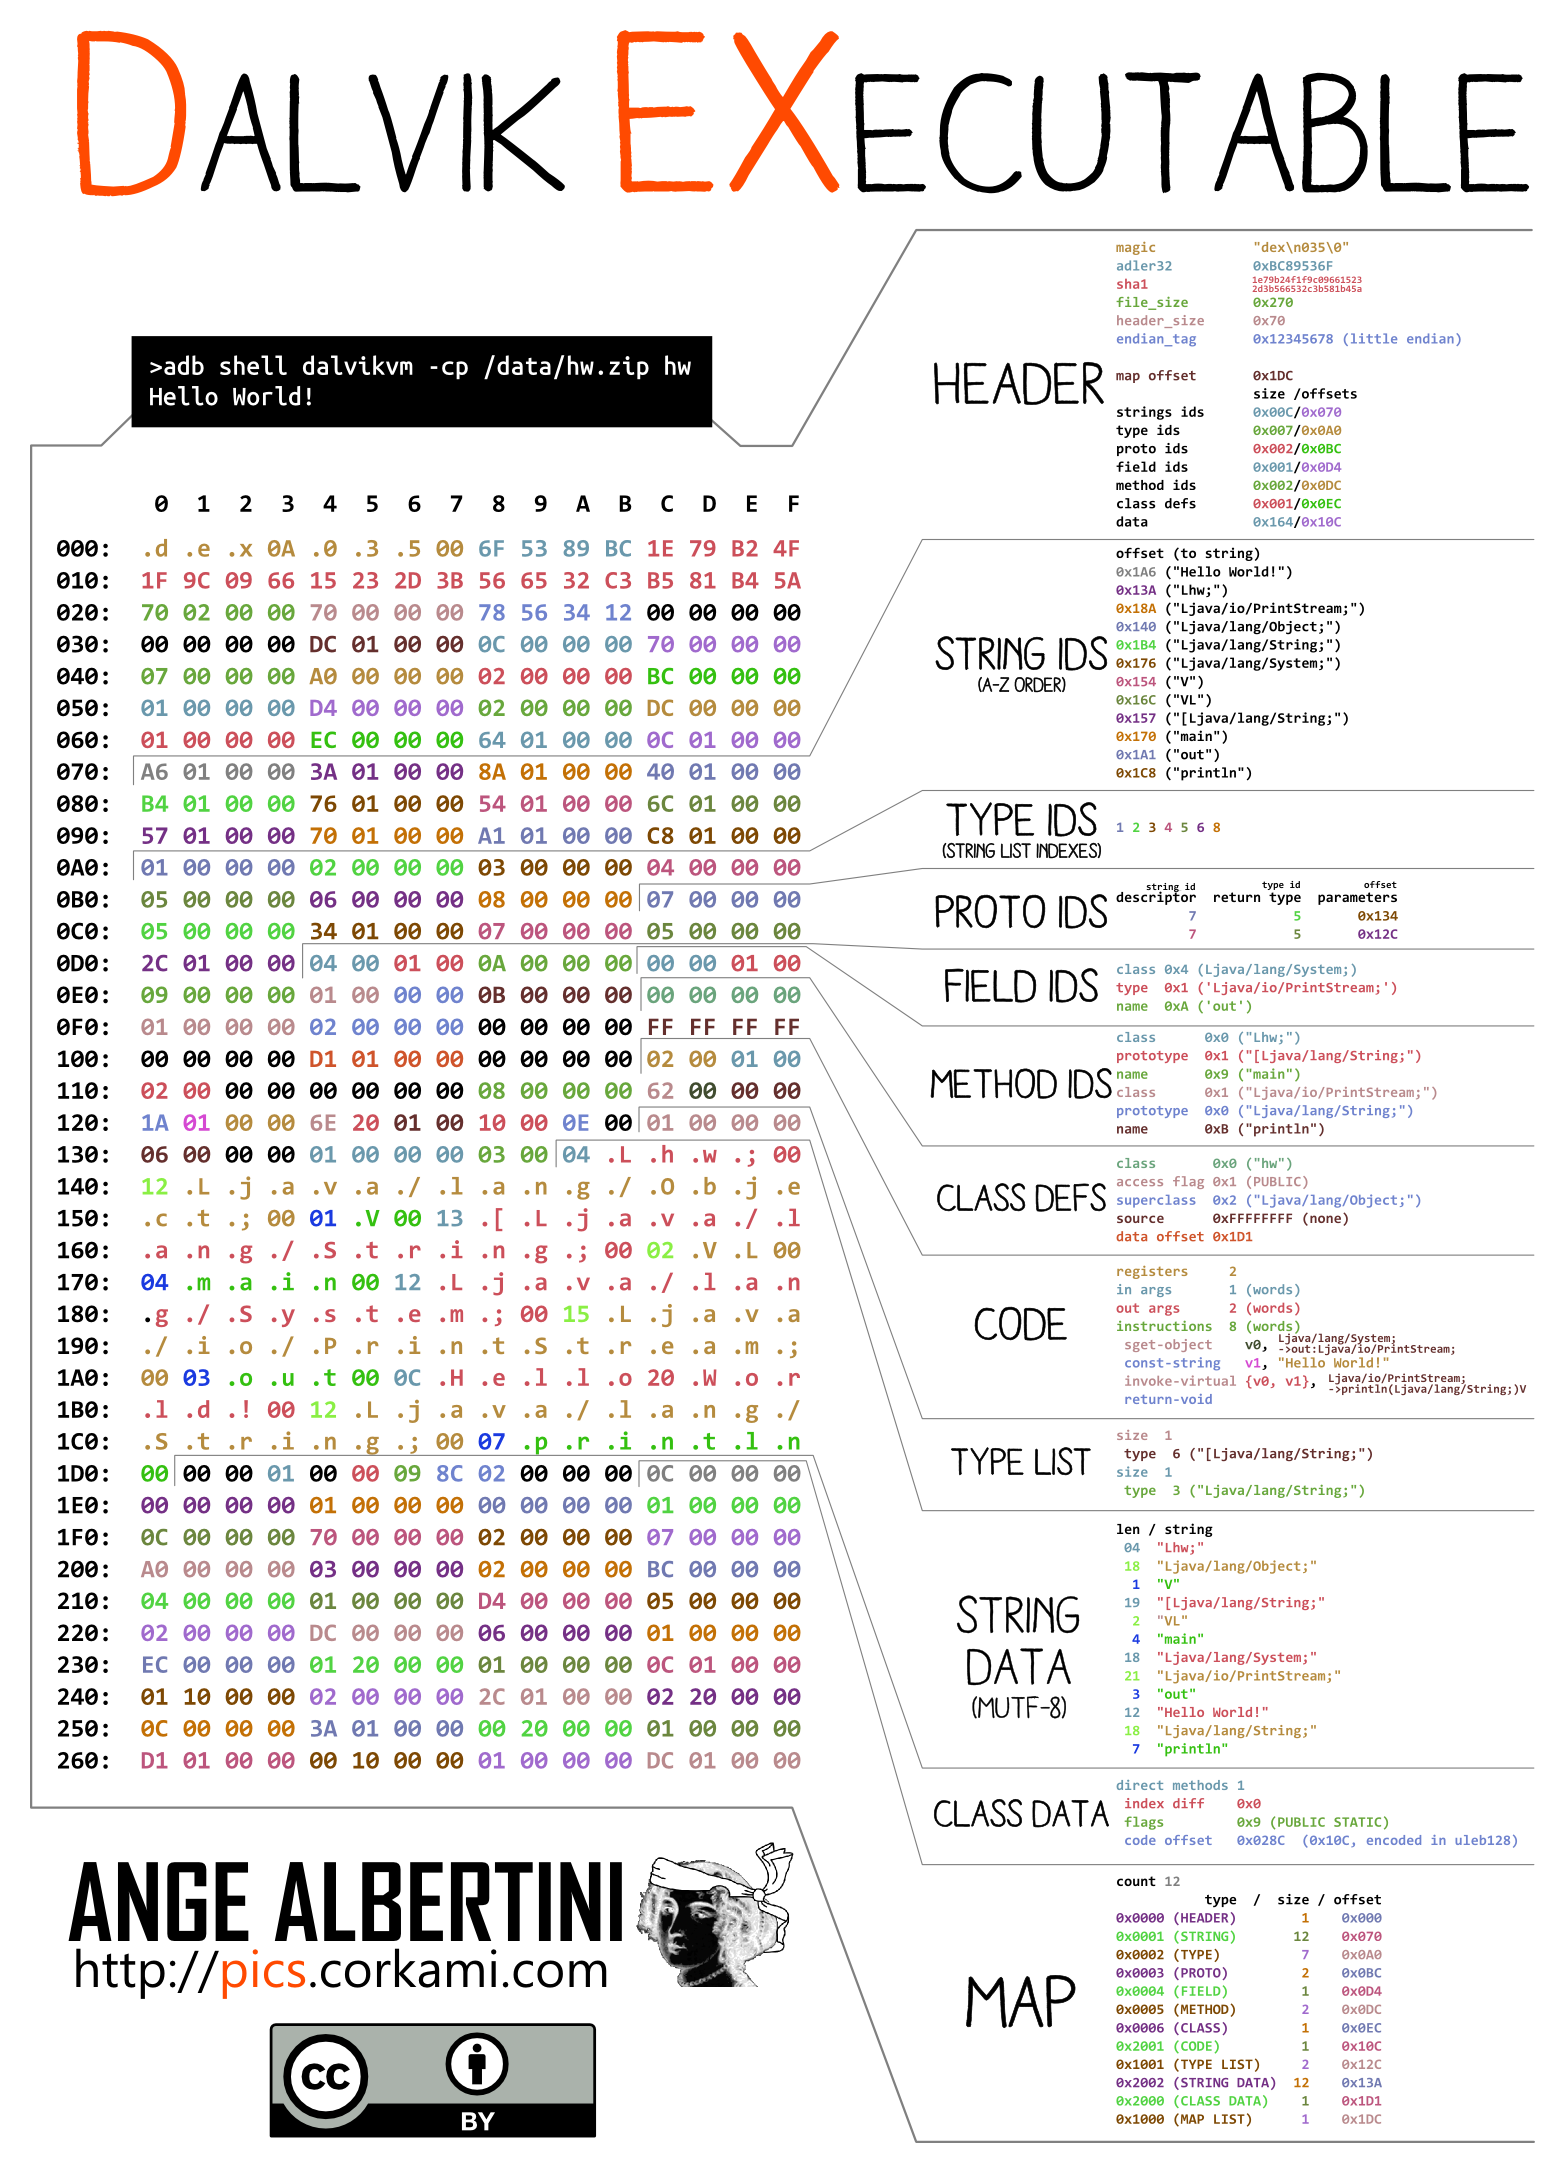
\includegraphics[width=\textwidth]{dex_format.png}
					\caption{Dex file format \cite{dex_image_albertini}}
					\label{fig:dex_format}
				\end{figure}
				
				\begin{longtable}{|l|l|p{7cm}|}
					\caption{Dex File Format}
					\label{table:Dex_file_format}\\		
					\hline
					\textbf{Name} & \textbf{Format} & \textbf{Description}\\
					\hline
									
					header & header\textunderscore item & The header contain information about how the dex file is organized, sizes of different sections inside the dex file, size of dex file, size of data section, version of dex format etc.\\
					\hline
					
					string\textunderscore ids & list of string\textunderscore id\textunderscore items & Its a list of string identifiers. These are identifiers for all the strings used by this file e.g, class names, method names, constant objects. Each item points to a location in data section (see below) where the original string is stored.\\
					\hline						
					
					type\textunderscore ids & list of type\textunderscore id\textunderscore items & This list contain type identifiers for all types (classes, arrays or primitive types) referred to by this file, whether defined in the file or not. The actual identifier string is stored in data section. Items in this list points to items in string\textunderscore ids list and which in turn points to type identifier string stored in data section.\\
					\hline
					
					proto\textunderscore ids & list of proto\textunderscore id\textunderscore items & Its a method prototype identifier list. Each item of this list contain three elements: \begin{itemize}
						\item \textbf{shorty\textunderscore idx} Points to string\textunderscore id\textunderscore item of shorty descriptor for this prototype
						\item \textbf{return\textunderscore type\textunderscore id} Specify return type by pointing to corresponding type\textunderscore id \textunderscore item
						\item \textbf{parameter\textunderscore off} Offset from start of file to the list of parameter types for this prototype. It must point to location in data section. The data there should be in "type\textunderscore list" format. This value would be zero in case no parameters.
					\end{itemize}\\
					\hline
					
					field\textunderscore ids & list of field\textunderscore id\textunderscore items & These are identifiers for all fields referred to by this file, whether defined in the file or not.\\
					\hline
					
					method\textunderscore ids & list of method\textunderscore id\textunderscore items & These are identifiers for all methods referred to by this file, whether defined in the file or not. \\
					\hline
					
					class\textunderscore defs & list of class\textunderscore def\textunderscore items & The classes must be ordered such that a given class's superclass and implemented interfaces appear in the list earlier than the referring class. Furthermore, it is invalid for a definition for the same-named class to appear more than once in the list. \\
					\hline
					
					call\textunderscore site\textunderscore ids & list of call\textunderscore site\textunderscore id\textunderscore items & These are identifiers for all call sites referred to by this file, whether defined in the file or not.\\
					\hline
					
					method\textunderscore handles & list of method\textunderscore handle\textunderscore items & A list of all method handles referred to by this file, whether defined in the file or not. This list is not sorted and may contain duplicates which will logically correspond to different method handle instances. \\
					\hline
					
					data & unsigned bytes & Containing all the support data for the tables listed above. Different items have different alignment requirements, and padding bytes are inserted before each item if necessary to achieve proper alignment. \\
					\hline
					
					link\textunderscore data & unsigned bytes &  The format of the data in this section is left unspecified by this document. This section is empty in unlinked files, and runtime implementations may use it as they see fit.\\
					\hline	
				\end{longtable}

			\subsection{Multiple Dex files in single APK}
				\paragraph{}  Android app (APK) files contain executable bytecode files in the form of Dalvik Executable (DEX) files, which contain the compiled code used to run your app. The Dalvik Executable specification limits the total number of methods that can be referenced within a single DEX file to 65,536 — including Android framework methods, library methods, and methods in your own code. This limit is referred to as the '64K reference limit' \cite{multidex}.
				
				\paragraph{} Versions of the platform prior to Android 5.0 (API level 21) use the Dalvik runtime for executing app code. By default, Dalvik limits apps to a single classes.dex bytecode file per APK.Multidex support library can be used to workaround this limitation. Android 5.0 (API level 21) and higher uses a runtime called ART which natively supports loading multiple DEX files from APK files Because of this support its not uncommon these days to come across APKs that contain multiple dex files e.g, Facebook, instagram etc. \cite{multidex}
		\section{Malware Analysis}\label{sec:malware_analysis}
		\paragraph{} Malware anaylsis is done to understand the behavior of malware sample, to come up with steps to avoid or remove the malware from infected systems, identify the threat actors, determine indicators of compromise (IOCs), Points of Interest(POIs) etc. There are main two categories of malware analysis:
		\subsection[Static Analysis]{Static analysis} In this category, we analyze the file by looking at its source code. This source code can be obtained by decompiling the sample and then looking for interesting patterns in this code like some well know strings, signatures, commonly used malicious code sections etc. This type of analysis doesn't give us any information about which code is executed and which code is not(dead code). It is also not good in analyzing samples that download the payload and the sample only the agent. There are different ways to compensate for the drawbacks discussed above like data flow analysis, taint analysis etc but that are beyond the scope of this report. For Android one of most popular static analysis tool is Androguard \cite{desnos2017androguard}..
		\subsection[Dynamic Analysis]{Dynamic Analysis} In this category of analysis the sample is executed in a controlled environment to see what malware is doing when executed. Which kind of network traffic it generates, which files does it interacts with, which system functions does it use. There are some challenges that this method of analysis faces like Emulator detection and delayed execution. For android the most popular dynamic anaylsis tool is CuckooDroid \cite{cuckoodroid_github}.
		
		\paragraph{} Both of the above categories have their own limitations but are widely used in hybrid mode. A malware analysis system use both of these on the sample to extract information. CuckooDroid uses Androguard along with insrumentation framework "Xposed Framework" to perform analysis. In coming chapters we will talk in more details about these two categories and how we used it in our analysis tools \cite{cuckoodroid_github}.
		
		\todo[inline]{To be done later, In this chapter we include the problem statement, See fh kiel project report structure for missing parts.}

\end{document}